\chapter{QUICK Box}
\label{chp:quickrollout} 

The main purpose of our study was to create an easy way to utilize the Mesh Potatoes in emergency situations and other situations where there are need for cheap and instant communication. Our main focus has been on providing Internet access to the mesh network, and the aspect of quick roll-out of the network. Internet access may be a vital way of communication in emergency situations, or just convenient in other situations. The process of setting up a mesh network providing Internet should be done quickly, since time is a crucial factor to consider in emergency situations. In this chapter we will describe parts of the set-up techniques for the Mesh Potatoes. Further on we will present our \gls{quick} Box, which is a box including a \gls{mp}, telephone, solar panel, battery and a charging regulator. A box ready to go in any situations. We will describe how we made this box, and similar work that have been conducted previously on the area. When it comes to the quick roll-out, specific approaches for making a best practice for quick roll-out will be presented. We will present the different types of up-links available to provide the mesh network with Internet access, along with a manual on how to connect the network to the different up-links. At last we will describe some situations where the need for a quick roll-out of a communication system may be needed. 

A big part of our work is gathering of information, and make this information more understandable for the common user. The existing user guides tend to be advanced and not adapted to people with little background knowledge on the area. Therefore we found it necessary to make the descriptions easier and more user friendly. The set-up procedures we explain in this chapter can also be found elsewhere. 


\section{Set-up of the Mesh Potato}
The set-up process of the Mesh Potato includes, among other activities, installing firmware, allocating \gls{ip}-addresses and providing Internet to the network. The firmware used for the \glspl{mp} is called \gls{secn} Firmware \cite{ChoosingFirmware}. 

\subsection{Configuring the Mesh Potato}
\label{subsec:configuring}
Configuring a Mesh Potato is the process of allocating an unique \gls{ip}-address to the \gls{mp}. Each of the \glspl{mp} were assigned a static \gls{ip} address, these addresses were not part of the \gls{lan} address space. The \gls{ip} addresses are allocated in a predefined default address space 10.130.1.20. In order to change this \gls{ip} address, the \gls{mp} has to be connected via an Ethernet cable to a PC running Linux. The PC must be on the same subnet as the \gls{mp}, in order to establish contact. When the PC is on the same subnet, the \glspl{mp} web interface can be accessed via a browser. In the web interface, the \gls{ip} of the \gls{mp} can easily be changed. This description works for both versions of the \gls{mp}. One difference is that you can change the \gls{ip} on \gls{mp1} by using \gls{ivr} commands (see page 28 in Appendix \ref{chp:appendixB}). A second version of the \gls{mp2} is in development. This version has a telephone jack port (\gls{fxs} daughterboard), which allows for \gls{ivr}. 

\begin{enumerate}
\item Set the PC to have the same subnet, by writing the following command in the terminal:
\noindent
\begin{lstlisting}[language=bash]
  $ ifconfig eth0 10.130.1.120 netmask 255.255.255.0
\end{lstlisting}
\item Open a browser and type in "10.130.1.20". The web interface will then appear. 
\item In the web interface, under network, change the \gls{ip} address field to "192.168.1.x", where x is the unique number for the specific \gls{mp}. This number should be between 21-99. In order to set the change, a save and reboot must be done from the interface. 
\end{enumerate}

\subsection{Upgrading the Mesh Potato}
\label{subsec:upgrading}
The firmware of the Mesh Potatoes are under constant development. It is therefore advisable that the \gls{mp} is running the latest version of the firmware. The process of upgrading the firmware is different from \gls{mp1} and \gls{mp2}. The different methods are described below. 

See the \gls{secn} User Guide for respectively \gls{mp1} and \gls{mp2} in Appendix \ref{chp:appendixB} and \ref{chp:appendixC} for a more detailed description of how to upgrade the firmware on the Mesh Potatoes.

\subsubsection{Installing Firmware on Mesh Potato 1.0}
Flashing is the process of updating or changing the firmware (\gls{secn}) on the \gls{mp1}. The most common way to perform the flashing process is by using the potato-flash application \cite{flashing}. This is a specialised software application for the Mesh Potato. Potato-flash can be used regardless of previously installed firmware on the Mesh Potato \cite{InstallingSecnFirmware}. 

\begin{enumerate}
\item Downloaded the 64 bit potato-flash utility from \url{http://download.villagetelco.org/utilities/potato-flash/potato-flash-64bit/} to the folder \textbf{/etc/local/bin}.
\item Made the potato-flash file executable by writing the following command in the Linux terminal.
\begin{lstlisting}[language=bash]
  $ cmod +x /usr/local/bin/potato-flash-x64
\end{lstlisting}
\item Downloaded the rootfs file (\texttt{openwrt-secn1_1-GA01-MP01-root.suashfs}) and the kernel file (\texttt{openwrt-secn1_1-GA01-MP01-vmlinux.lzma})  from \url{http://download.villagetelco.org/firmware/secn/stable/mp/SECN-1.1/} to a folder we called mp\_firmware in our local directory.
\item Opened the terminal and wrote the following commands: 
\end{enumerate}


\begin{framed}
\noindent \textbf{Enter root environment:} 
\begin{lstlisting}[language=bash]
  $ sudo su
\end{lstlisting}

\noindent \textbf{Turn of network manager:}
\begin{lstlisting}[language=bash]
  $ service network-manager stop
\end{lstlisting}

\noindent \textbf{Bring the interface connected to the \gls{mp} up:}
\begin{lstlisting}[language=bash]
  $ ip link set eth0 up
\end{lstlisting}

\noindent \textbf{Go into the directory containing the .squashfs and .lzma files:}
\begin{lstlisting}[language=bash]
  $ cd <the directory containting the .squashfs and 
  .lzma files>
\end{lstlisting}

\noindent \textbf{Assign IP-address to the interface:}
\begin{lstlisting}[language=bash]
  $ ifconfig eth0 1.1.1.1
\end{lstlisting}

Before running the potato-flash utility we made sure that the \gls{mp} was unplugged from its power supply, and that the Mesh Potato was connected to our PC via an Ethernet cable. 

\noindent \textbf{Executing the potato-flash utility:}
\begin{lstlisting}[language=bash]
  $ potato-flash-x64 openwrt-secn1_1-GA01-MP01-root.suashfs 
   openwrt-secn1_1-GA01-MP01-vmlinux.lzma
\end{lstlisting}
\end{framed}

Briefly after the potato-flash had been executed, dots stared appearing on the screen, like shown in \fref{fig:flashing}. When these dots started appearing, we plugged the power supply back into the Mesh Potato, and the process of upgrading the firmware started. 

\begin{figure}[t]
  \centering
      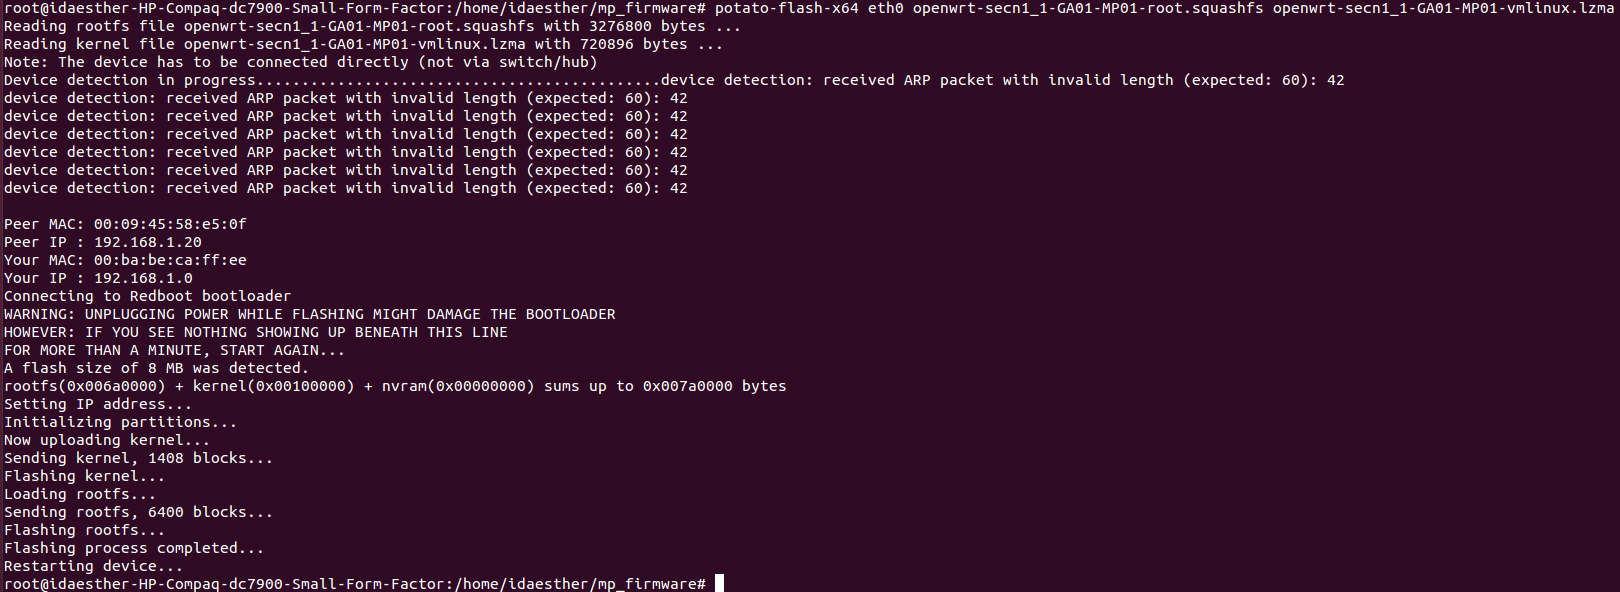
\includegraphics[width=1\textwidth]{potatoFlash.png}
  \caption [Flashing the Mesh Potato]{\textbf{Flashing the Mesh Potato.} This figure shows the flashing process from when we first flashed our Mesh Potato 1.0}
  \label{fig:flashing}
\end{figure}


\subsubsection{Installing Firmware on Mesh Potato v2.0}
The process of upgrading the MP's firmware is simplified with the \gls{mp2}. With the \gls{mp1}, command shell must be utilized in order do this. In contrary, with the \gls{mp2}, firmware upgrade can be done from the \gls{secn} web interface (more information about the interface can be found in section \ref{subsec:interface}). Extra functionality has been added to the interface from \gls{mp1} to \gls{mp2}. Under "Advanced" in the interface an extra tab called "Firmware" is added, and there the firmware upgrade can be executed. When this button is pressed, a new windows pops up where you have to add the firmware file. The firmware for \gls{mp2} can be found here: \url{http://download.villagetelco.org/firmware/secn/unstable/mp02/SECN-2.0/SECN-2.0-RC4/}.

\subsection{The SECN Web Interface}
\label{subsec:interface}
Village Telco provides a SECN web interface for configuration and management of individual \glspl{mp}. This web interface can be accessed by entering the \gls{ip} address of the \gls{mp} in a browser, this interface is shown in \fref{fig:webinterface} In order to be able to do this, the PC must be on the same subnet (exact same prefix) as the \gls{mp}.  

The web interface allows the user to do alterations in the \gls{mp}. The web interface allows the user to alter some key parameters. Among these are changing the \gls{ip} address of the device, set up the WiFi \gls{ap}, \gls{voip}/\gls{sip} Configurations, Password and Web Server Security. The web interface also allows the user to do changes to more advanced settings and monitoring. To get a detailed description of the web interface see the user guide in Appendix \ref{chp:appendixA}. In addition to this, like mentioned above, the interface has been extended and improved from \gls{mp1} to \gls{mp2}. More actions can be conducted via the interface with \gls{mp2}. 

\begin{figure}[t]
  \centering
      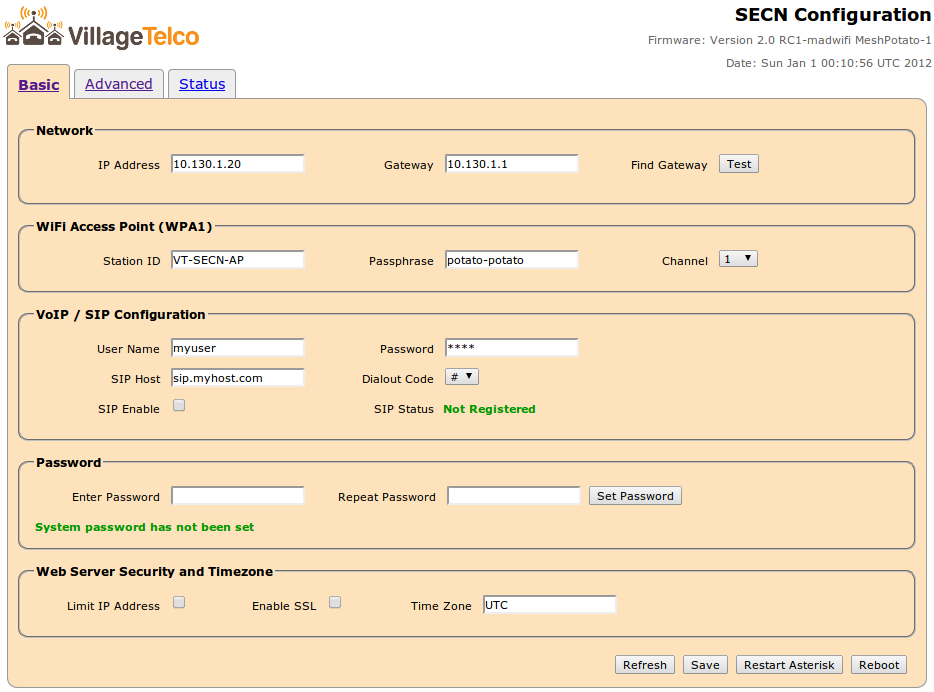
\includegraphics[width=1\textwidth]{webinterface.png}
  \caption [Web interface]{\textbf{Web interface.} Displays the web interface to the Mesh Potato.}
  \label{fig:webinterface}
\end{figure}

\section{QUICK Box}
The Mesh Potatoes and Village Telcos were created to get voice and data connection to areas where services like these are non existent or too expensive for the average person. As of now the Mesh Potatoes have been set up to create small or bigger networks in villages all over the world. We want to expand this solution by looking at its mobility and its usage on the go. We want to make a box that has high adaptability, enabling it to easily be used in several different scenarios, under different conditions and by different people, all with different needs. The box have to be so easy that there are no room for misunderstanding or mistakes. It should be a to-go box ready for any situations.  
 
\subsection{Previous/similar work}
\paragraph{Go Box.} Something similar has been done before by Keith Williamson, a volunteer in the Village Telco community. His idea of utilizing the Mesh Potatoes in emergency situations started with his interest in amateur radios, and the use of radios in emergency situations. He put together a "go box" by using a waterproof Pelican 1200 case. This case contained a bracket holding the Mesh Potato, a rechargeable Li-Ion or Li-Poly battery, telephone handset and junction box to provide an on/off switch \cite{keith}. Our Emergency Box differ in some ways from the Go Box made by Williamson. 

\paragraph{AfrikaBurn.}
AfrikaBurn is a "Burning Man" festival in Tankwa Town in the Karoo (South Africa) that is held once a year \cite{whatisafrikaburn}. This is a festival with focus on art and freedom of expression. Instead of using money, the festival attendants are inspired to trade different types of goods with each other. A Village Telco has been established at this festival a few years now. Free-standing phone boots with Mesh Potatoes powered by solar panels has been set up at the festival area. The first year five phone boots where set up around the festival area. Since it were few numbers to call, the calling became sort of random. This gave a  "ChatRoulette" like effect, only with phones instead. The second year some aspects where improved from the previous year. The boots had production \glspl{mp}, no lighting and new sleeves. A netbook was brought with them, and this acted as a gateway \cite{africaburnforavillagetelco,africaburnsagainforavillagetelco}. 

\paragraph{Millitary}
* høre med Arild om hvas om brukes i millitæret i dag, om det er noe liknende i det hele tatt

\subsection{Key Components}
The key components of our emergency box is described in \tref{tab:components}. 

\begin{center}
\begin{table}[h!]
\caption{\label{tab:components}The components of Emergency Box}
    \begin{tabular}{ | l | p{9cm} |}
    \hline
    \textbf{Component} & \textbf{Description and purpose} \\ 
    \hline
    Access point for Internet &  Mesh Potato v2.0\\ 
    \hline
    Suitcase/box &  A suitcase made of high quality plastic coated with aluminium foil. Strengthened edges and corners of aluminium and steel. It has a soft-padded interior, than can be split into different rooms. Two snap locks with keys, and a solid handle for carrying. Dimensions: 455x330x152 (width, depth, height). Weight: 2,6 kg. \\ 
    \hline
    Power supply & A gel battery (12 V and 5 Ah). No need for maintenance. The battery acid is bound in a viscous gel. This prevents leakage, even when the battery is mounted horizontally. Long lifetime and safe to handle. The battery is fully closed, and do not need refill of battery water. No hydrogen gas or other gas might leak. When the battery is charging no gas or acid vapor is emitted, hence the battery can be placed in narrow or enclosed spaces. The battery withstands multiple discharges. The gel battery is ideal for seasonal or occasional use, since it have a slow self-discharge tempo, and a good ability to recover after deep discharging. Dimensions: 114x69x109. Weight: 2,16 kg. \\
    \hline
    Plain old telephone &  A regular plain old telephone that can be connected to the \gls{mp1} via a \gls{fxs} port by using a RJ-11. \\
	\hline
	Solar panel & Solar panel from Multicomp with item number: MC-SP10-GCS. Power rating: 10 W. Power Voltage Max: 17 V. Dimensions: 357x280x18\\
	\hline
	Charging regulator & Regulator for 12 V solar panel. Protects the battery from overcharging and discharge. The charging regulator is connected between the solar panel and the battery to regulate the voltage to the battery. Capacity: 100 W / max. 7 A. Overcharging protection: 14.5 V. Discharge protection: <10,5 V. Three diodes shows charging, high voltage and low battery voltage. \\
	\hline
    \end{tabular}
   \end{table}
\end{center}

\subsection{Creating the QUICK Box}
This section describes how we created the \gls{quick} box from scratch. A go-box is delivered with everything already set up. The Mesh Potato is configured and delivered with an unique \gls{ip} address. The suitcase contains a cd with Linux Ubuntu in case the user does not already have it installed, and there would be a need for the user to configure or upgrade the \gls{mp}. The case would also contain necessary cables and detailed descriptions on how to connect to the different up-links. \fref{fig:boxinmaking} shows the box in the making.

\begin{figure}[t]
  \centering
      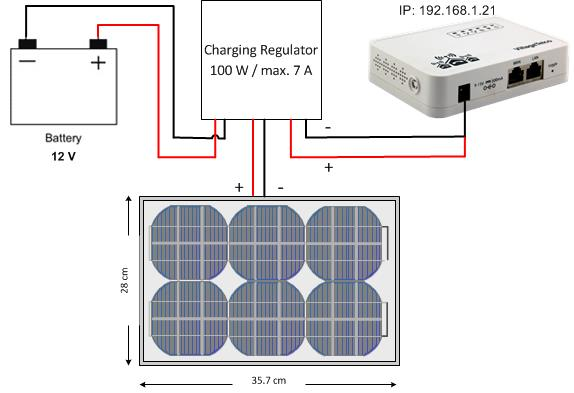
\includegraphics[width=0.9\textwidth]{emergencybox.jpg}
  \caption [The composition of the \gls{quick} box]{\textbf{\textbf{The composition of the \gls{quick} box.}} This figure shows how the key components in the \gls{quick} box is conjoined together.}
  \label{fig:emergencybox}
\end{figure}

\paragraph{Conjoining the components of the QUICK box.}
The components that we used to construct the box was a solar regulator, a gel battery, a solar panel and a Mesh Potato. These components were put together as shown in \fref{fig:emergencybox}. The solar regulator is connected to all the components, and is used in order to not overcharge the battery. The solar regulator was initially built for another type of solar panel than the one we chose to use. This means that the concomitant plugs could not be used. These plugs were cut of and we soldered on our own wires.  

New wires were soldered on the solar regulator, one was connected to the power cord to the Mesh Potato, the other two fro, respectively, the battery and the solar panel. Before connecting everything together we used a multimeter in order to measure the voltage in the solar panel. We placed the solar panel under a bright lamp to see if it made any impact, which it did. We used the multimeter to check the battery as well, which was fully charged, with a voltage of a little over 13 V. 
We fist connected the solar panel, then the battery, and at last the Mesh Potato. In order for all to work the \gls{mp} have to turn on, which it did.  

\begin{figure}
        \centering
        \begin{subfigure}[t]{0.4\textwidth}
                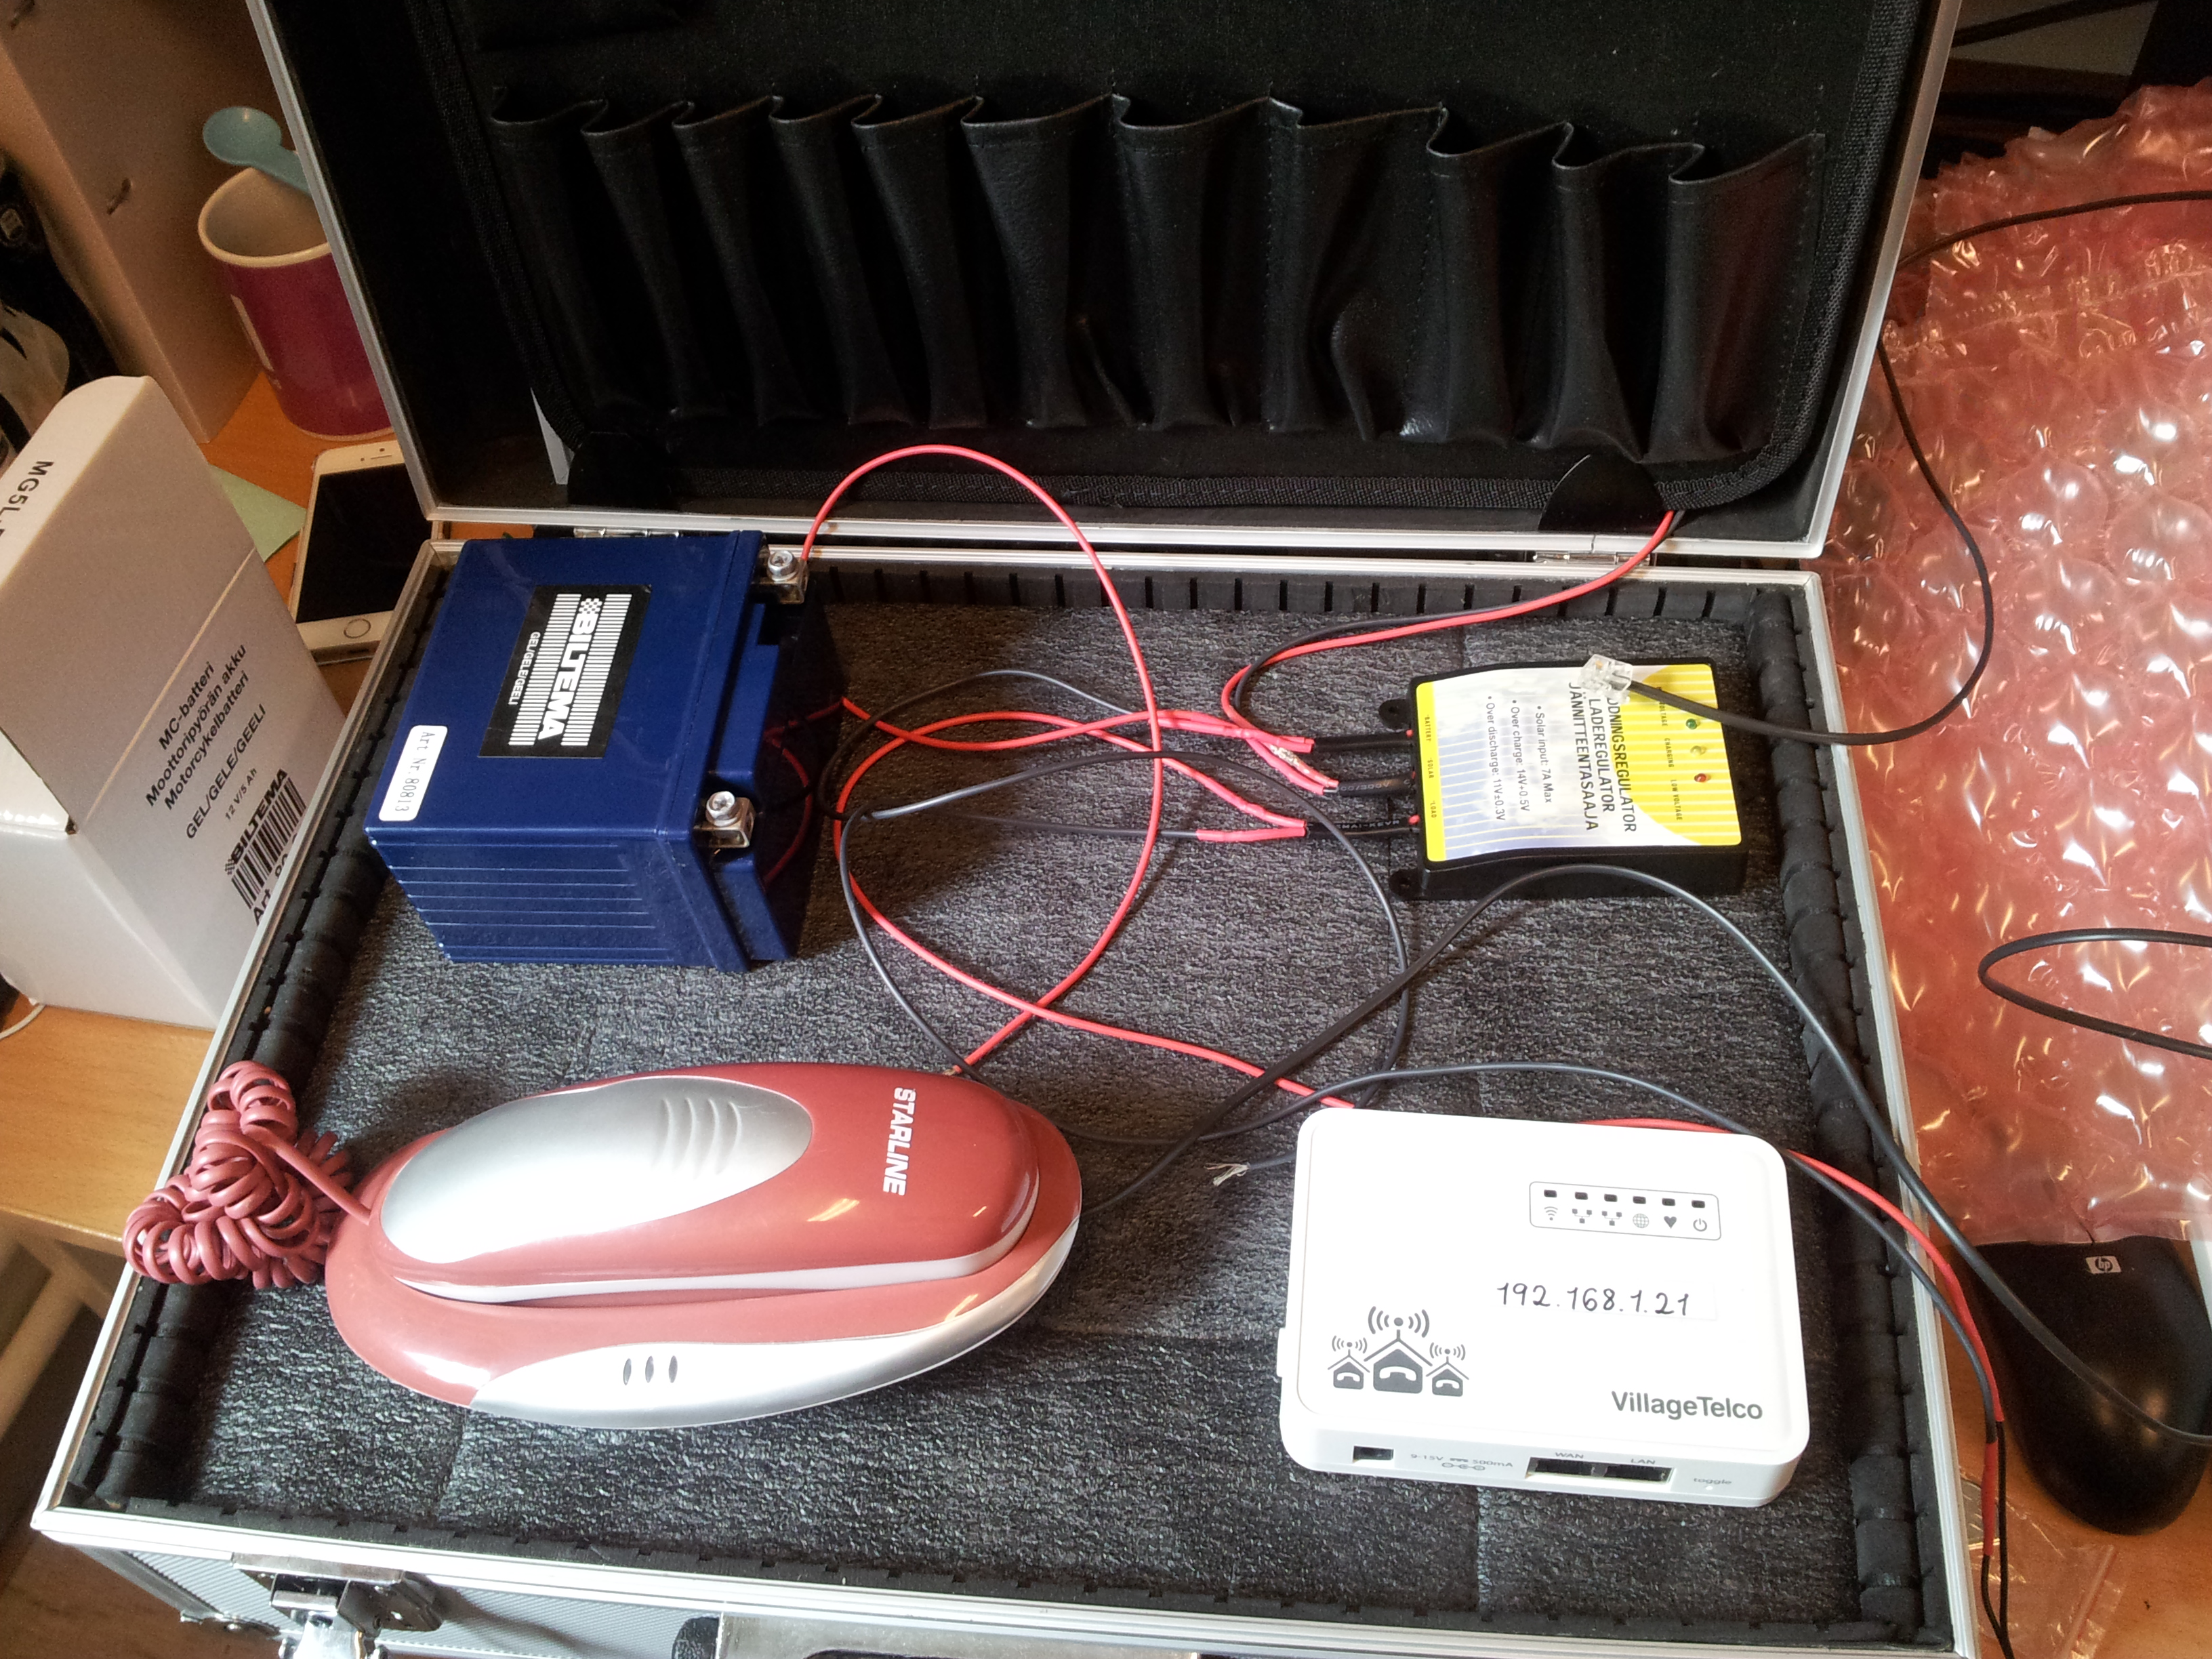
\includegraphics[width=\textwidth]{boxinmaking2}
                \label{fig:boxinmaking2}
        \end{subfigure}
        \begin{subfigure}[t]{0.4\textwidth}
                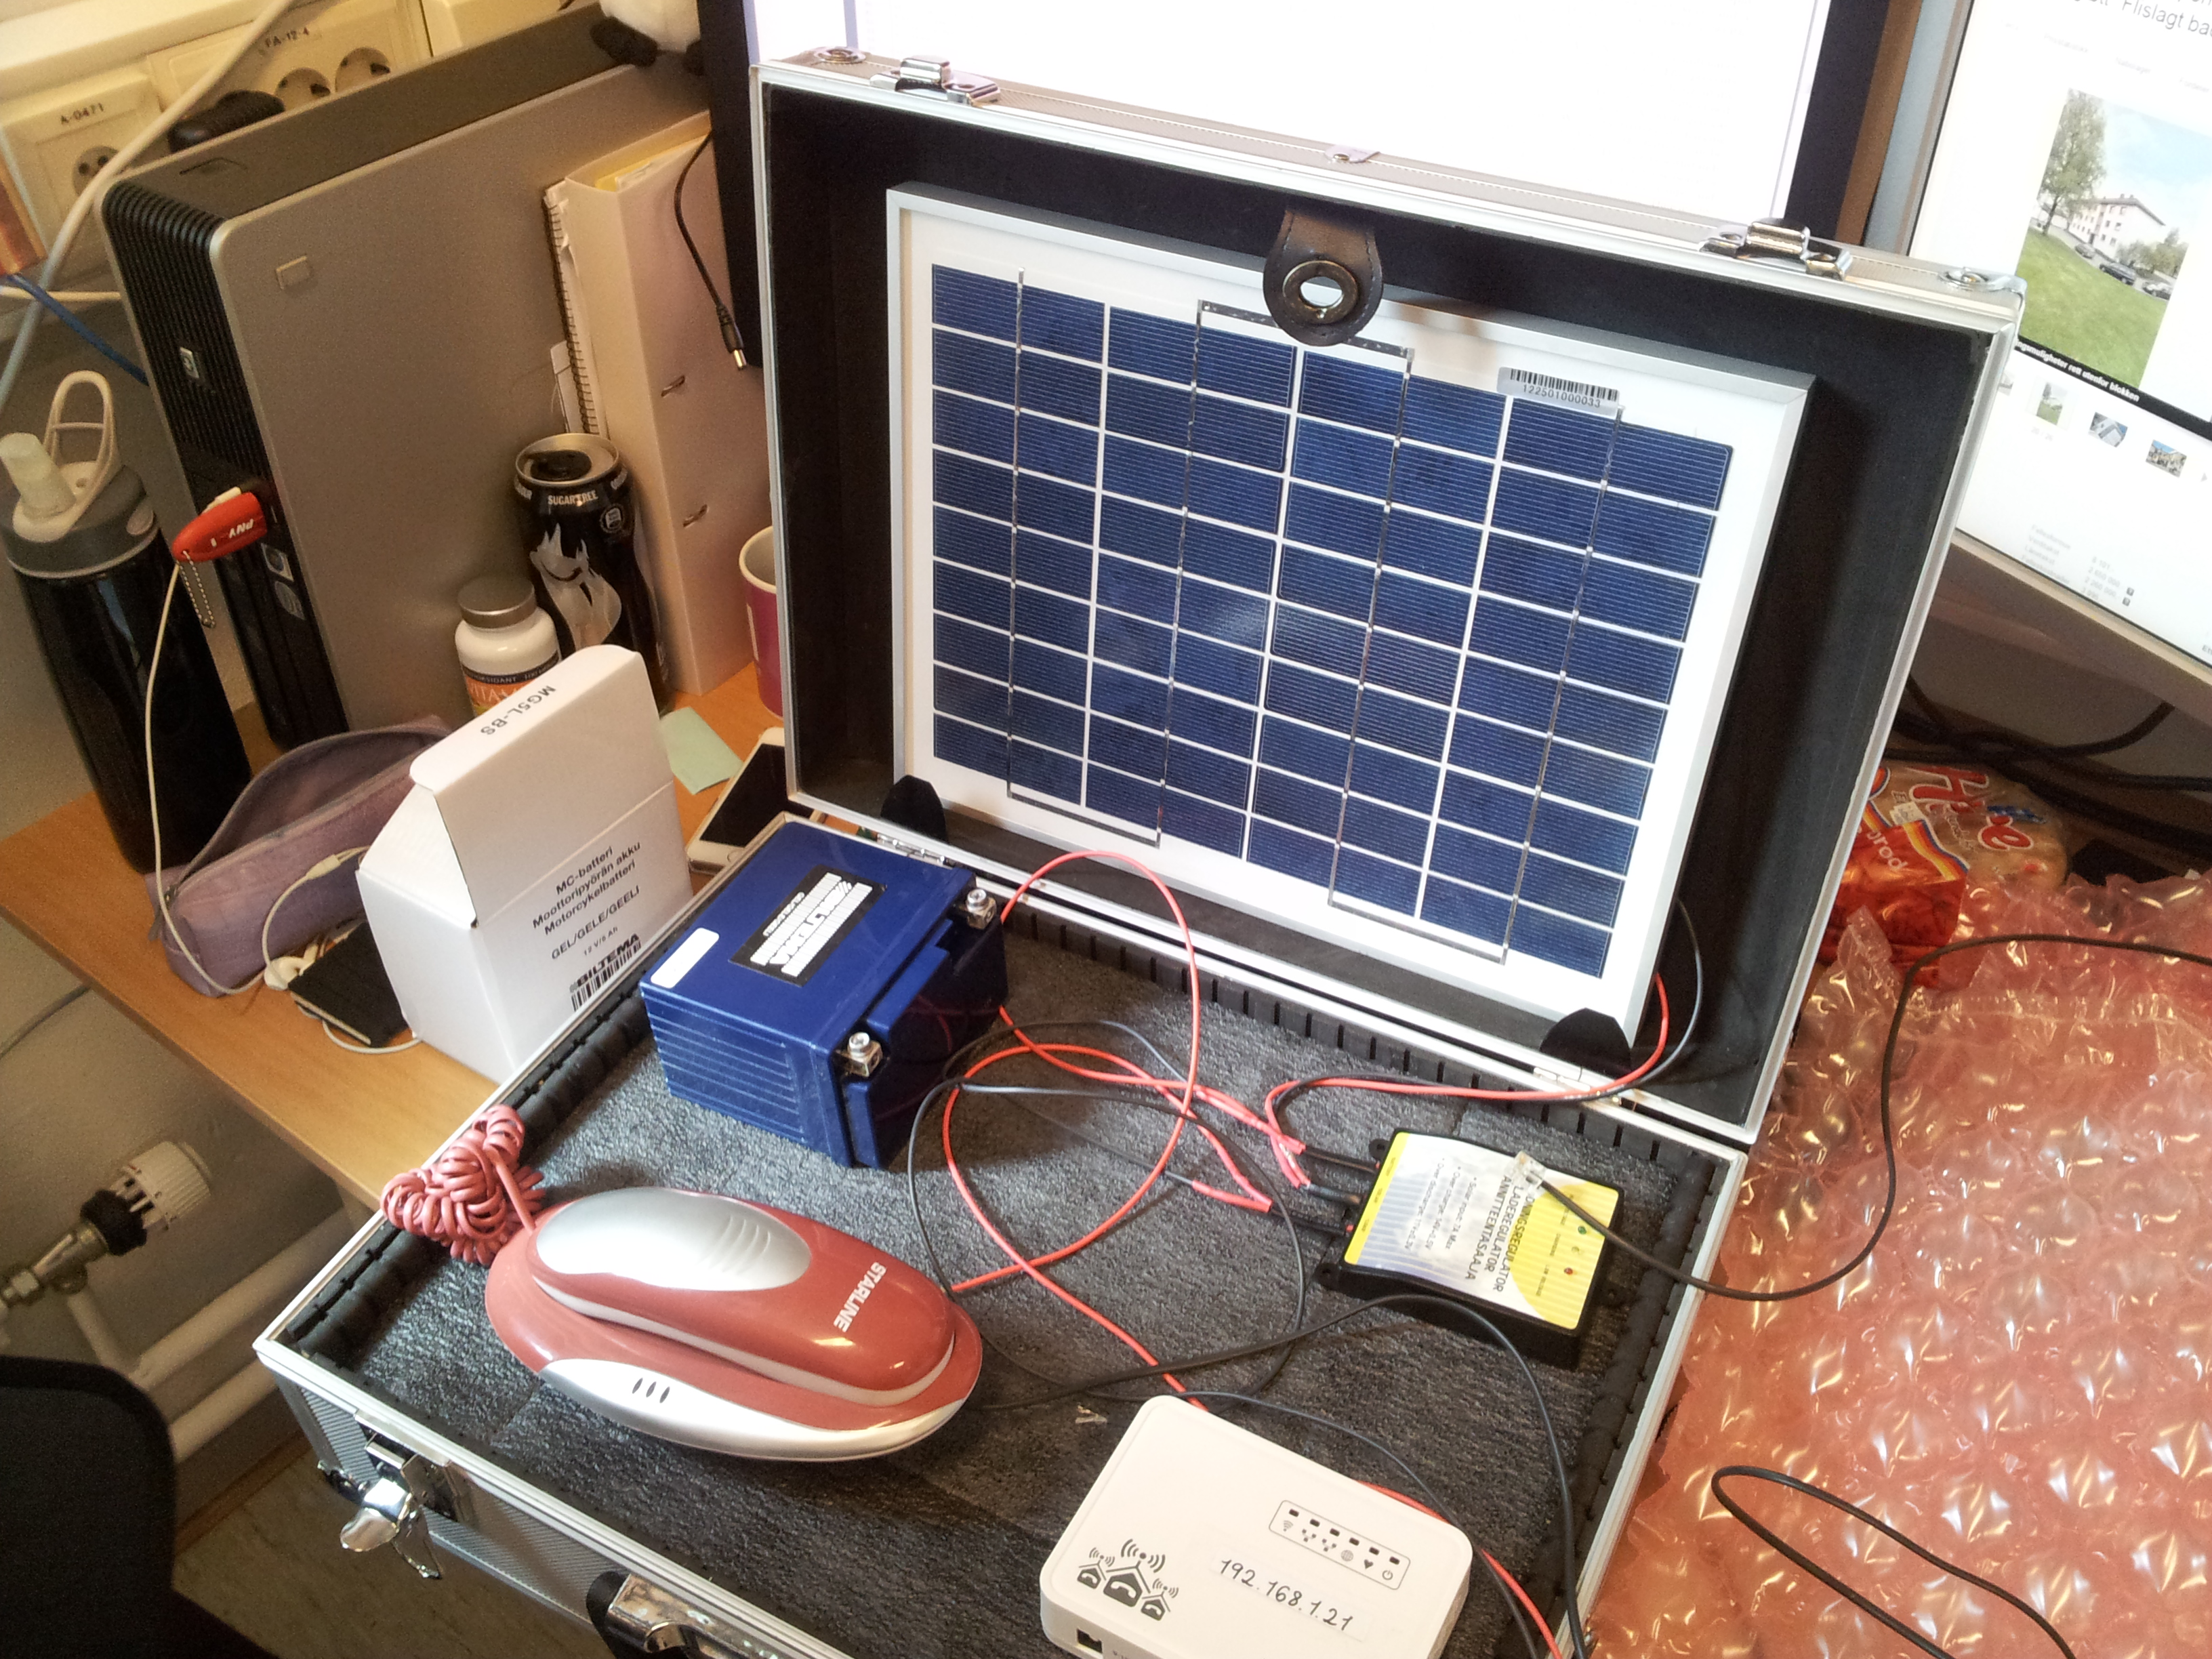
\includegraphics[width=\textwidth]{boxinmaking4}
                \label{fig:boxinmaking}
        \end{subfigure}
         \begin{subfigure}[t]{0.3\textwidth}
                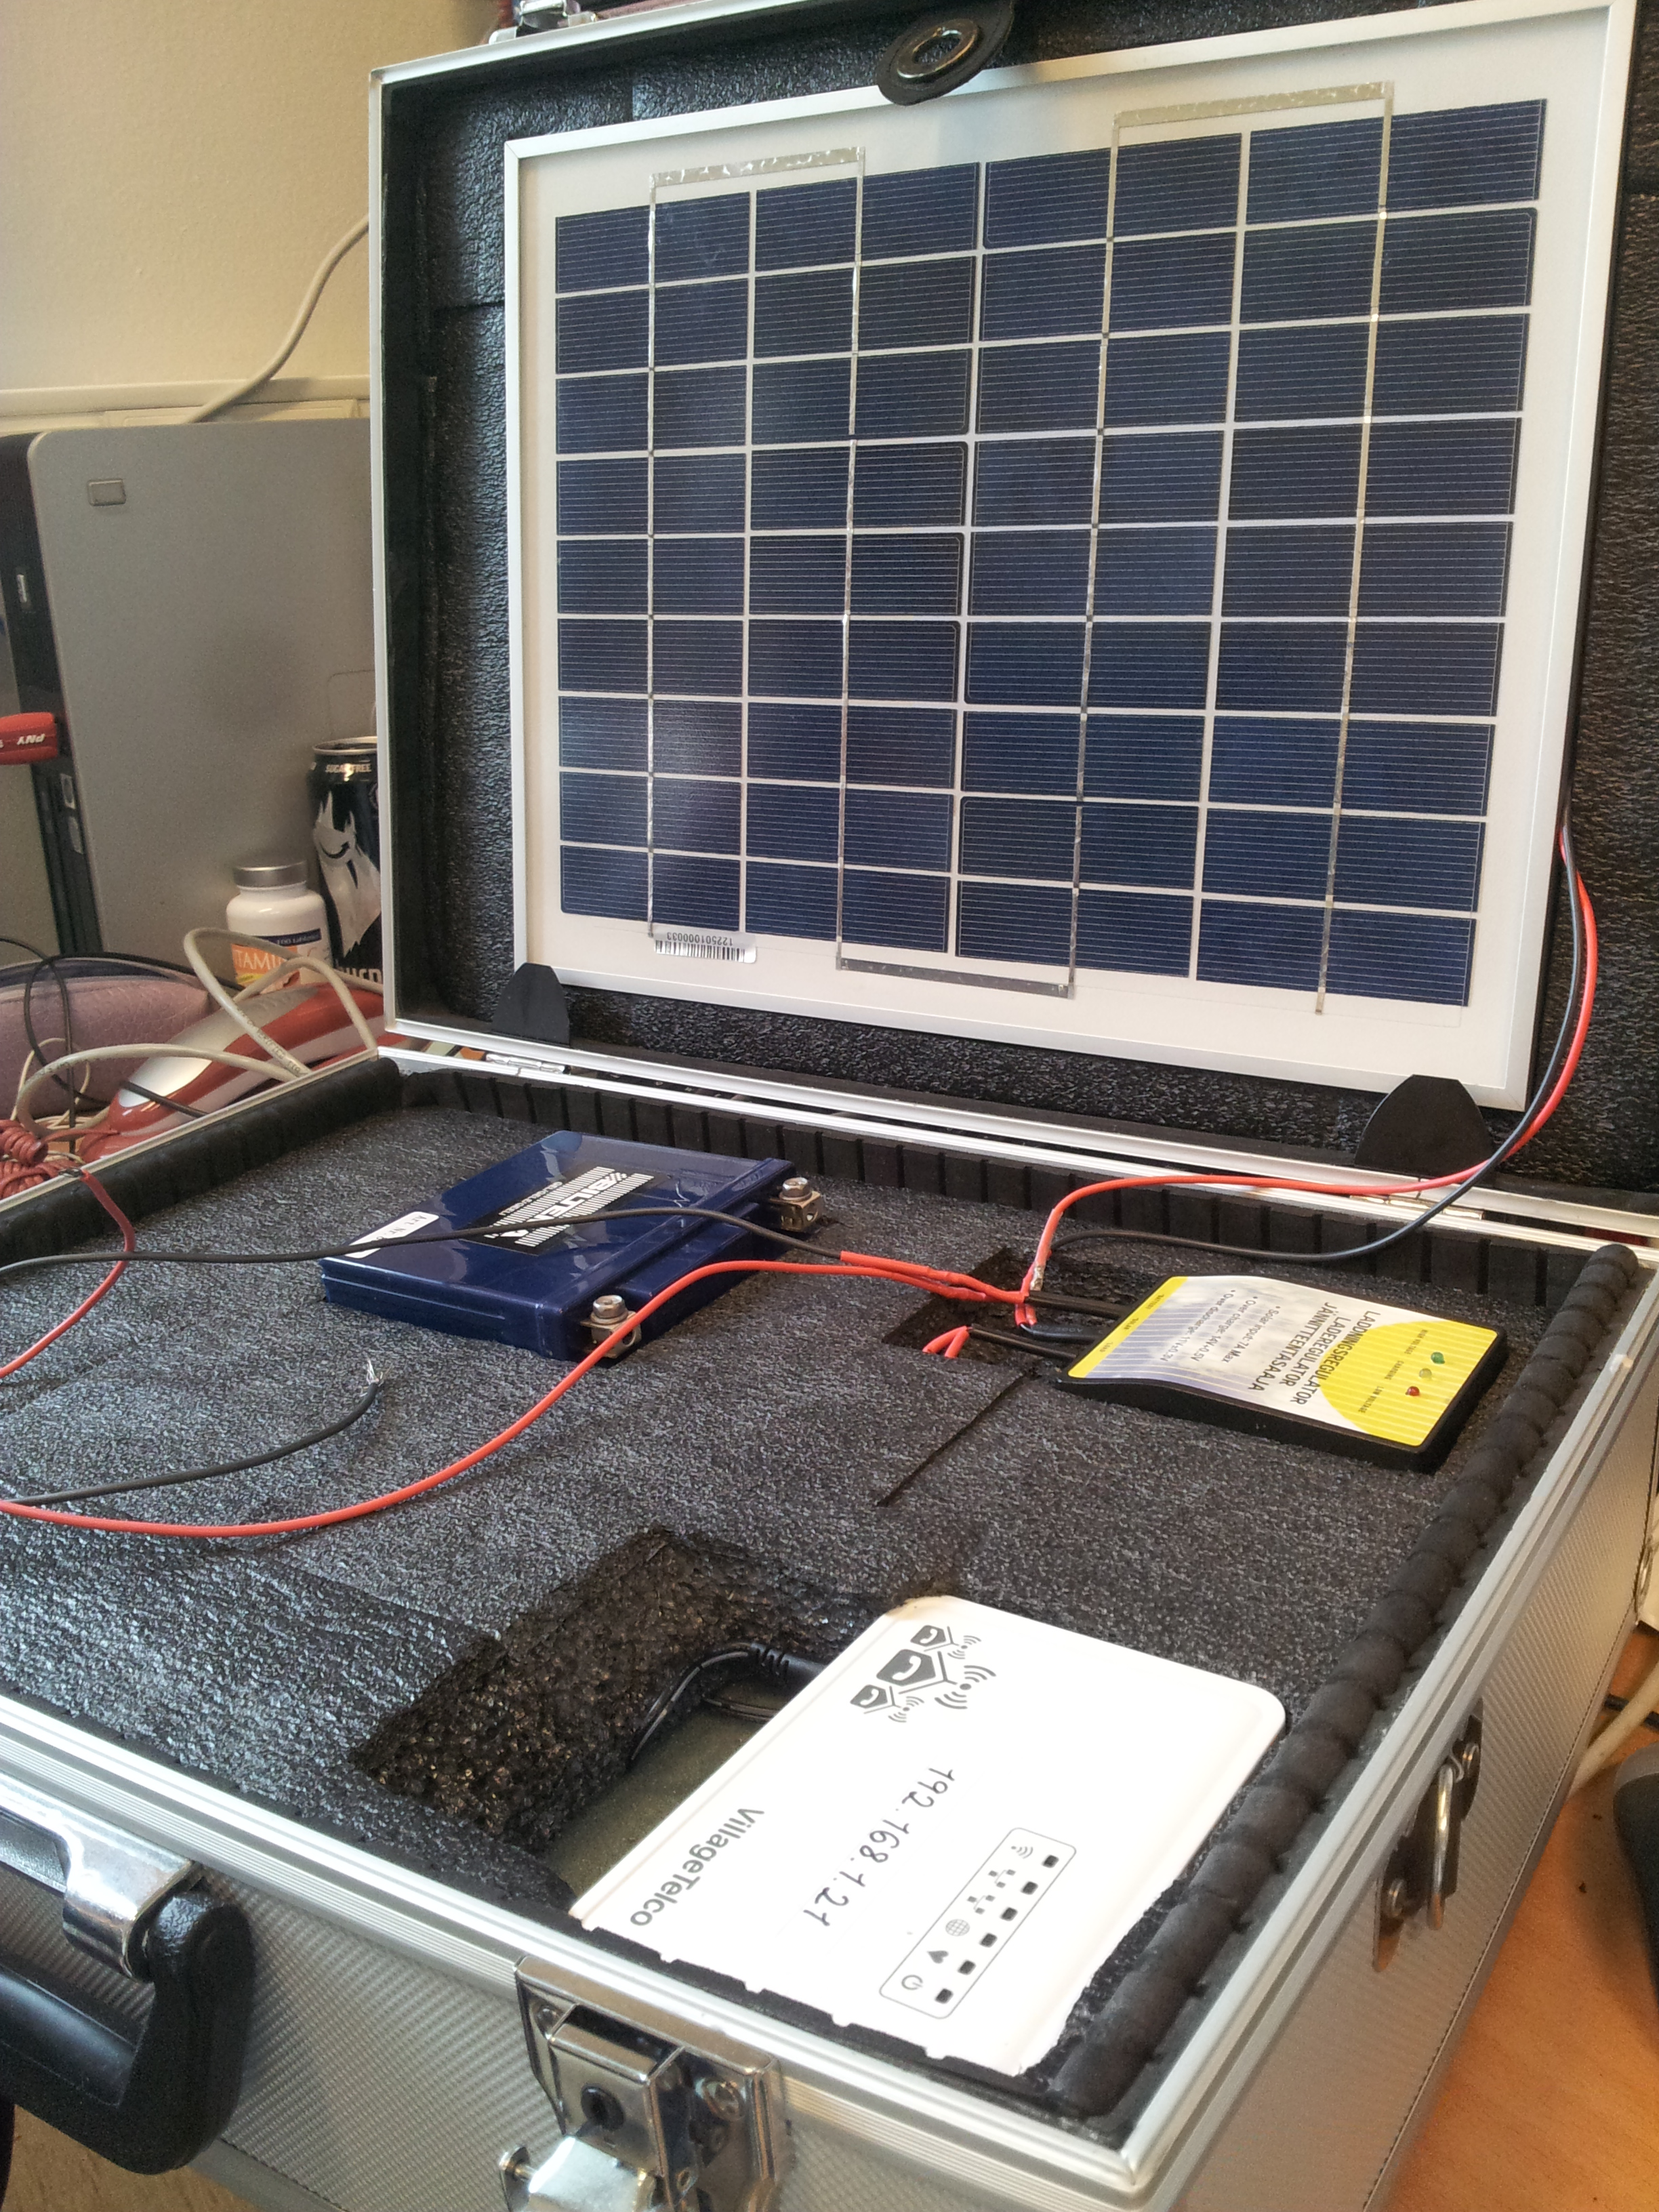
\includegraphics[width=\textwidth]{boxinmaking3} 
                \label{fig:boxinmaking3}
        \end{subfigure}
        \begin{subfigure}[t]{0.4\textwidth}
                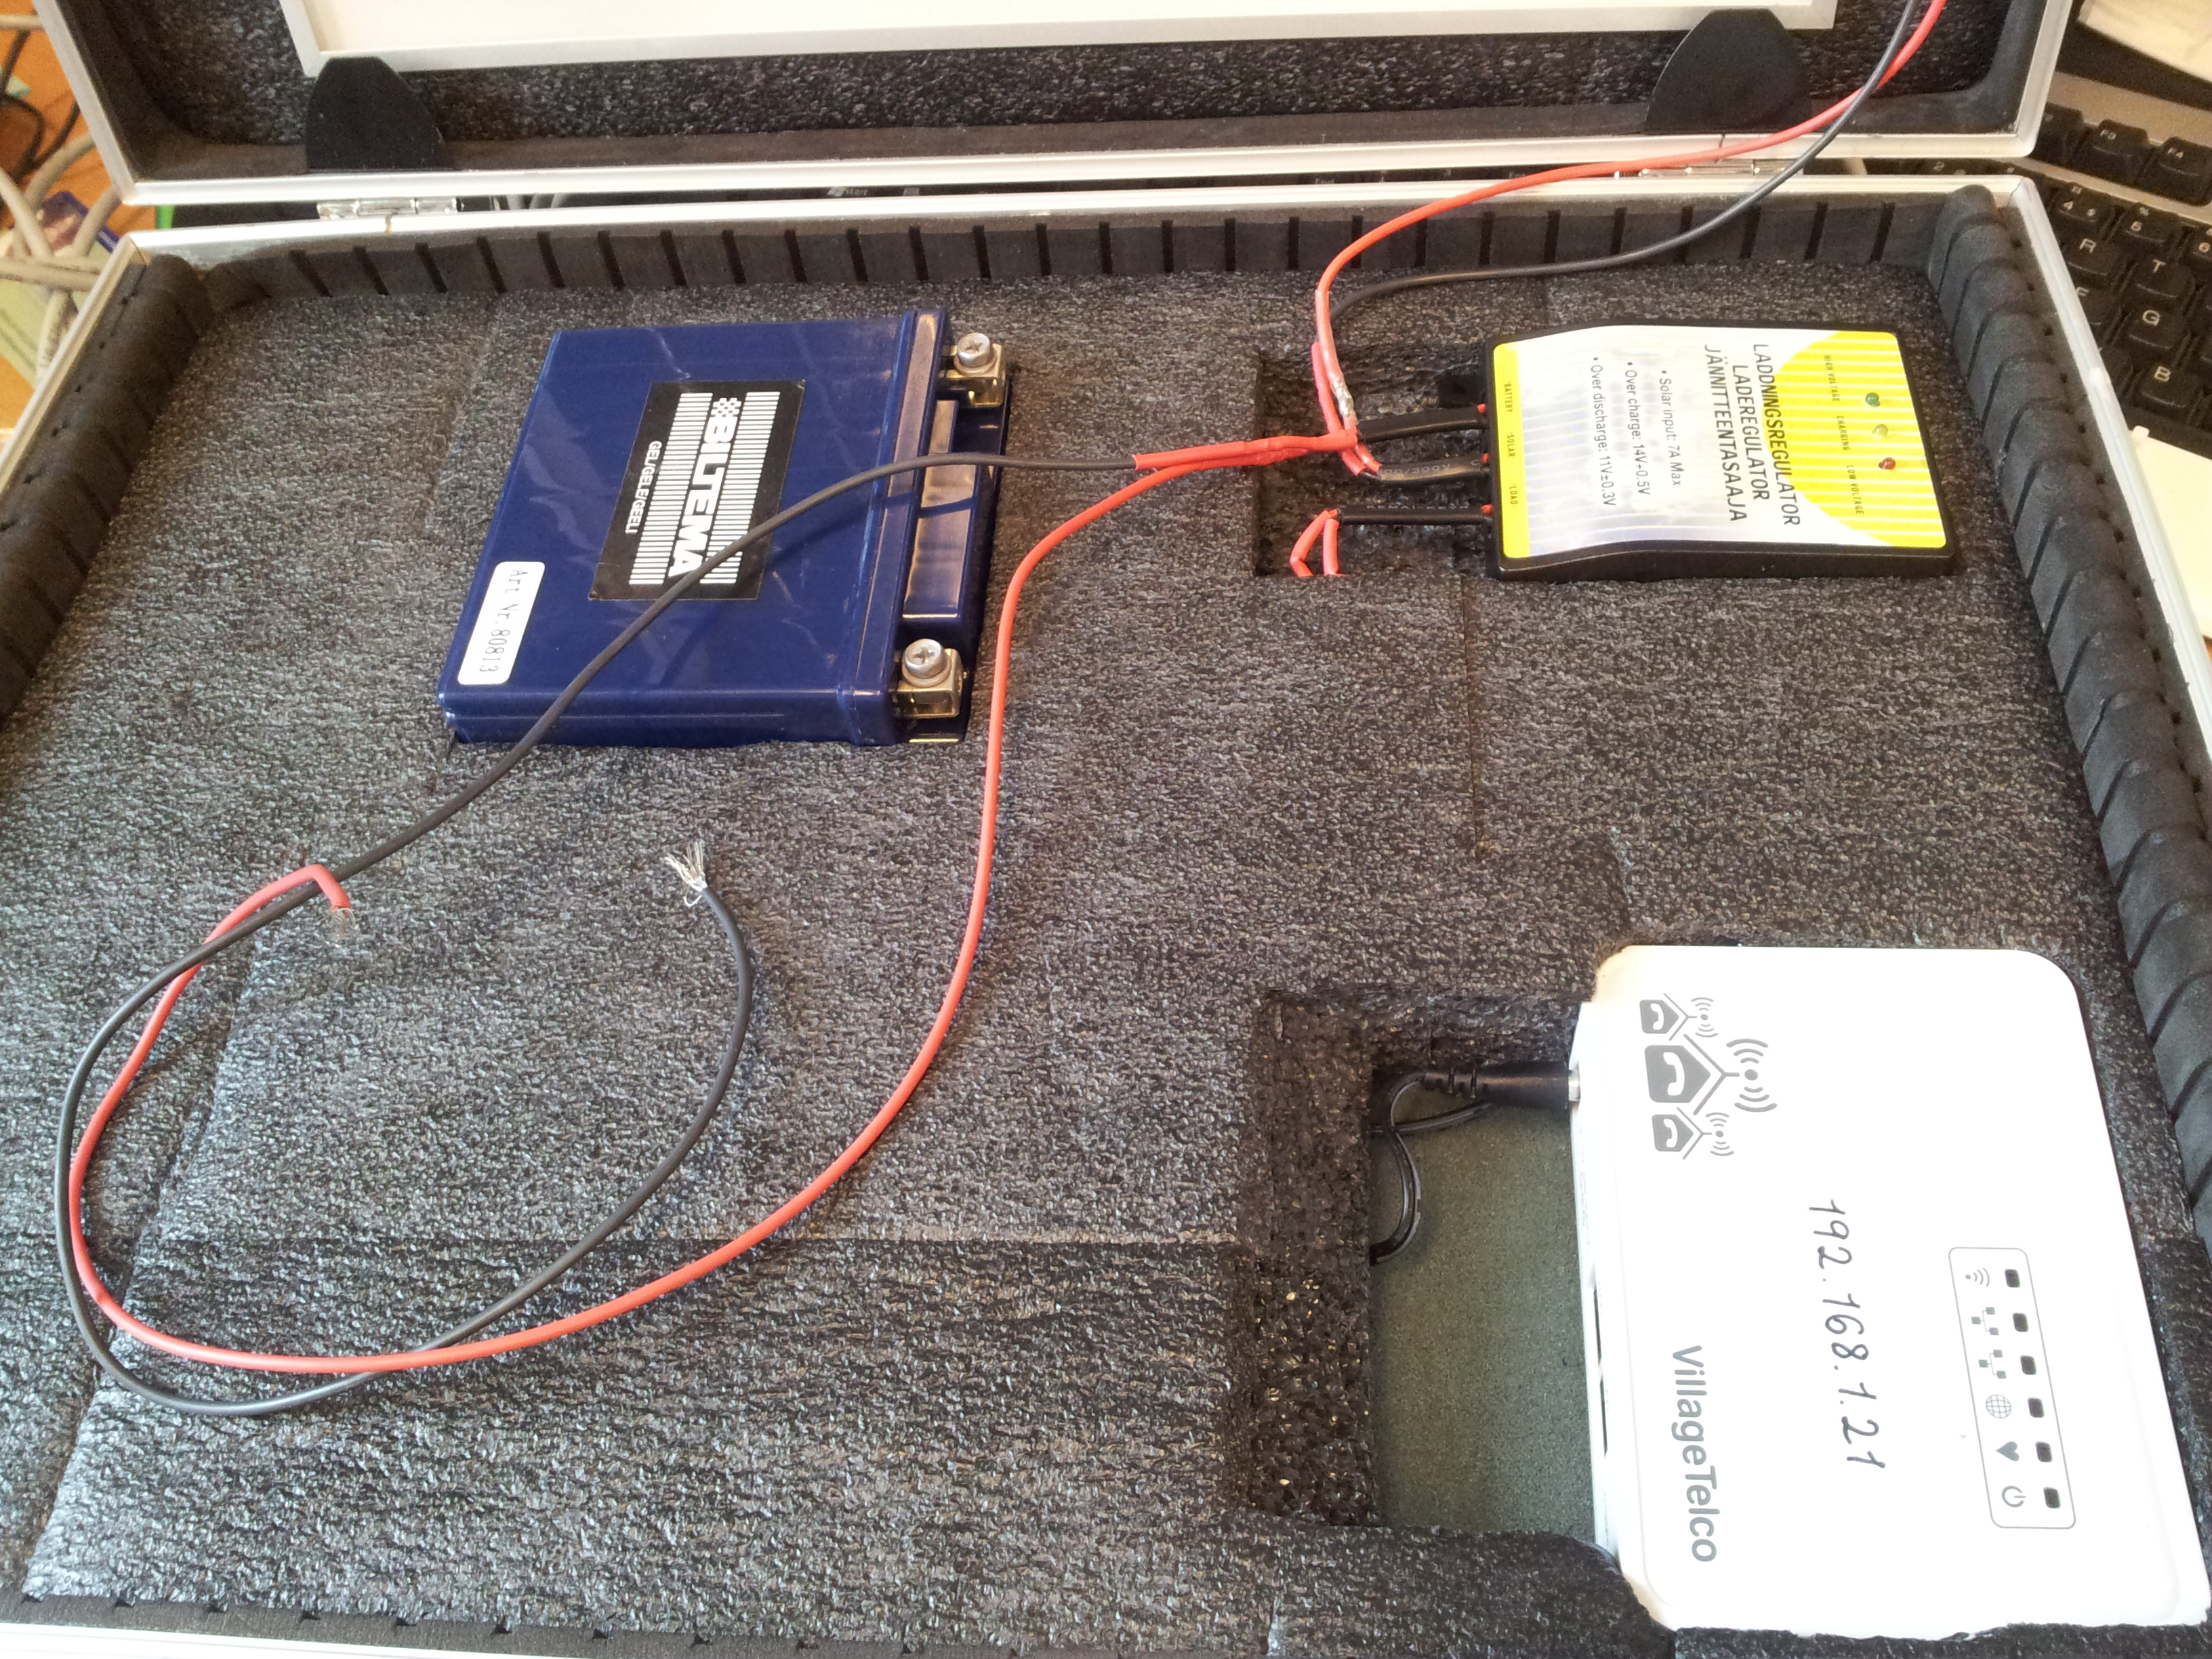
\includegraphics[width=\textwidth]{boxinmaking} 
                \label{fig:boxinmaking4}
        \end{subfigure}
\caption{The QUICK box in the making.} \label{fig:boxinmaking}
\end{figure}

\paragraph{Configuring and upgrading the QUICK Box}
When the \gls{quick} box is delivered the Mesh Potato is already set-up and configured with an unique \gls{ip}-address, and running the latest version of the \gls{secn} firmware. The descriptions will be in the box in case something would happen and there will be a need to upgrade or configure. These processes are described in sections \ref{subsec:configuring} and \ref{subsec:upgrading}.

\subsection{Battery and Charging Calculations}
All the calculations done in this section is based on the components described in \tref{tab:components}. 

\paragraph{Charging with solar panel.}
How long it will take for the solar panel to charge the battery from fully discharged to fully charged, depends on how much sun there is. The following calculations are calculated using the peak value of the solar panel (10W). 

The solar panel capacity is:
$$Amp = \frac{Watt}{Volt} = \frac{10 W}{17 V} = 0.59 Ampere$$

When charging batteries it is important to take the charging factor into account. This factor is the ratio between supplied capacity and submitted capacity. The charging factor varies depending on type of battery. For our gel battery the factor is roughly 1.2. The charging factor does not have an annotation. 
If the battery is completely discharged it will take: 

$$Amp\times Hours = AmpHours \Rightarrow Hours =\frac{AmpHours}{Amp} = \frac{5 Ah\times 1.2}{0.59 A} = 10.17 Hours$$

to fully charge it. 

This calculation does not take into consideration that the solar panel may have to charge the battery while the \gls{mp} is running. The effect from the solar panel to the battery will then decrease. 

\paragraph{Charge while MP01 is running.}
The capacity from the solar panel will then be: 
$$Amp = \frac{Watt}{Volt} = \frac{10-2.5 W}{17 V} = 0.44 Ampere$$

The time it will take to fully charge the battery from fully discharged condition will then be: 
$$Amp\times Hours = AmpHours \Rightarrow Hours =\frac{AmpHours}{Amp} = \frac{5 Ah\times 1.2}{0.44A} = 13.6 Hours$$

\paragraph{Charge while MP02 is running.}
The capacity from the solar panel will then be: 
$$Amp = \frac{Watt}{Volt} = \frac{10-0.75 W}{17 V} = 0.54 Ampere$$

The time it will take to fully charge the battery from fully discharged condition will then be: 
$$Amp\times Hours = AmpHours \Rightarrow Hours =\frac{AmpHours}{Amp} = \frac{5 Ah\times 1.2}{0.54A} = 11.1 Hours$$

Number of sun hours per day in for example South Africa in December is approximately 14. In June number of sun hours is approximately 10.5. And off course, it can be cloudy, so these numbers are best case. This means that it is possible to fully charge the battery in the course of a day, but it may not always be the case. The following calculations shows how long the battery can provide the Mesh Potato with power from fully charged condition without the solar panel charging it at the same time. 

\paragraph{On fully charged battery - MP01}
This calculation takes into account that the solar panel is disconnected from the battery. With the components described in \tref{tab:components} the number of hours the \gls{mp1} can last with fully charged battery is: 

$$Amp = \frac{Watt}{Volt} = \frac{2.5 W}{12 V} = 0.208 Ampere$$
$$Amp\times Hours = AmpHours \Rightarrow Hours = \frac{AmpHours}{Amp} = \frac{5 Ah}{0.208 A} = 24 Hours$$

\paragraph{On fully charged battery - MP02}
This calculation takes into account that the solar panel is disconnected from the battery. With the components described in \tref{tab:components} the number of hours the \gls{mp2} can last with fully charged battery is: 

$$Amp = \frac{Watt}{Volt} = \frac{0.75 W}{12 V} = 0.06 Ampere$$
$$Amp\times Hours = AmpHours \Rightarrow Hours = \frac{AmpHours}{Amp} = \frac{5 Ah}{0.06 A} = 83 Hours$$


\subsection{Possible Improvements}
As mentioned this set-up is fairly easy and simple, but leaves room for improvements. There should be an on/off switch to not use unnecessary battery capacity. This on/off switch would be placed between the battery and the regulator. Unless a measuring instrument is available to check the voltage, there are no way for the user to know the remaining battery time. This might be very useful in situations where communication is vital and the hours of battery lifetime are limited and should be taken into account. 

The battery we used is a gel battery. They are less explosive than the lithium batteries, and are better suited to be placed into enclosed spaces that may get hot. The downside of the gel batteries is their weight, they are heavy. Since our aim is to make a case that is portable, a lighter battery would be preferable. Under the requirement of being portable a factor to keep in mind is that it is not allowed to bring lithium batteries on the plane. This means that if we chose to use a lithium battery in our solution a regular person would not be allowed to bring their \gls{quick} box on the plane. in the case of relief organizations, this might not be a problem since they transport their equipment in special planes, like a hercules. 

The \gls{mp2} is a lot smaller than the first generation, and a powerful solar panel does not take that much space, so there is no need for a suitcase of the size we have purchased. A smaller case that is lighter and easier to handle would make the solution even more portable. 

Our main focus was to get something that worked and that was safe, and we did not focus on aesthetics and appearance. This is therefore also an area where there are room for improvements. 


\section{The Process of Quick Roll-Out}
As mentioned, one of our areas of focus is the process of quick roll-out. There are many aspects that can be included in order to speed up the roll-out process and make it as easy as possible. We will now present some of our ideas to meet this requirement.

\subsection{Script}
A script is a list of commands that can be executed without user interaction, in other words, to automate a process. In order to connect the mesh network to Internet a list of commands have to be executed. One idea to speed up the process of setting up the network was to create a script to automate this process. One way to do this could be by creating a self-executable script that could be included in the \gls{quick} box on for example on an USB-stick. There would have to be a different script, and different USBs, for each up-link type. 

We made a script that simplifies the process of getting Internet to a Mesh Potato via a PC (see section \ref{subsec:internetviaPC} for step-by-step description) with wireless Internet connection. This script can be found in Appendix \ref{chp:appendixD}. The PC was running Linux Ubuntu and had a wireless Internet connection. Some easy steps must be conducted to run the script:
\begin{enumerate}
\item Make sure the \gls{mp} is connected to the PC via Ethernet cable.
\item In the terminal go to the directory where the script is located and enter the following command:
\noindent
\begin{lstlisting}[language=bash]
  $ sudo su
  $ sh scriptviaPC.sh
\end{lstlisting}
\end{enumerate}


\subsection{With the MP02}
The \gls{mp2} Basic does not have the option to connect to a phone. Hence the issue with telephone number distribution is irrelevant. Later in 2014 Village Telco will release a new version of the \gls{mp2}, \gls{mp2}-Phone. MP2-Phone will be identical to \gls{mp2} Basic, just with an \gls{fxs} daughterboard. With this new version the issue of number distribution appears. 

The \gls{quick} box could be delivered with several \glspl{mp}, where each \gls{mp} is marked with the pre-configured IP address. Since it is not possible to connect a phone to the \gls{mp} there is no issue of number distribution. The box could for example contain 5 \glspl{mp}, where one would be connected to an up-link, while the other ones would be strategically placed in order to spread the Internet access further. 

\subsubsection{Distributing Numbers}
When a Village Telco is set up today, telephone numbers are distributed by updating a spreadsheet with name and number to the users. These spreadsheets are printed out and delivered to everyone. This is a system that might seem cumbersome, but serves its purpose. If new nodes are added to the network or any changes are made, new sheets have to be printed out and delivered to everyone. This way of spreading telephone numbers might be more difficult with the go-box. 

One option is to continue with the number distribution approach in use today. The suitcase could contain 5 \glspl{mp}, all \glspl{mp} are marked with its unique \gls{ip} address. There will be attached a list with the \gls{ip} addresses of the other Mesh Potatoes in the suitcase. When setting up the network the names can easily be filled in on each Mesh Potato. This will then be the telephone list.  

Another approach would be to integrate the distribution of phone number in the web interface. A new feature could be implemented in the interface. This feature would discover the other \glspl{mp} in range, also in range through other \glspl{mp}. All \glspl{mp} would be displayed with name of the \gls{ssid}, \gls{ip} address, where the last octet is the telephone number and the name of residence or user. This name could be edited by the master user or by the user themselves. Each \gls{mp} in the suitcase are pre-configured and set up, they are also set up with security and a password to enter the web interface. So in order for a user to enter the web interface they have to enter the password to get access. Once inside they can see other \glspl{mp} in range and also put in their name for the other \glspl{mp} to see. The password and security is set up so that no other than the main user of the \gls{mp} can change the name. 


\subsection{Get Started - How to Use the Box}

This is a description of how you set up and get started with the \gls{quick} box. 

Make sure that the \gls{quick} box contains all these items: 
\begin{itemize}
\item A Mesh Potato
\item A battery
\item A solar panel
\item A charging regulator
\item Ethernet cable
\item A CD with Linux Ubuntu operating system
\item A USB-stick containing a script called "scriptviaPC.sh"
\item Descriptions on how to connect the Mesh Potato to different uplinks in order to provide Internet access. 
\end{itemize}

The \gls{quick} box is delivered with a pre-configured Mesh Potato, and a fully charged battery. The battery can be charged by placing the solar panel in sunlight. 

\begin{description}
\item[] \textbf{Name of Mesh Potato (SSID):} MP2_21.
\item[] \textbf{IP address of the Mesh Potato:} 192.168.1.21
\item[] \textbf{Password:} potato-potato 
\end{description}

The password is the default password used on Mesh Potatoes, and it can be changed in the user interface for a more secure option. The SSID can also be changed there if that is preferable. 

To set up the \gls{quick} box: 
\begin{enumerate}
\item Connect the wires to the battery (the red one to plus and the black one to minus). The Mesh Potato should then automatically turn on. 
\item To provide Internet to the mesh network, follow the attached descriptions for the specific uplink type you have available. 
\end{enumerate} 

In order to preserve the lifetime of the battery, it can be smart to disconnect the wires from the battery while the box is not in use. A fully charged battery has a lifetime of approximately 83 hours. This is when the solar panel is not connected to the battery. Take into consideration that the charging time when the battery is completely discharged is approximately 10 hours. If the \gls{mp2} is connected while charging, 1 hour is added to the charging time. 


\subsection{How Connect the MP02 to Cabled Internet}
\label{subsec:cabledInternet}
\subsubsection{Quickly Connect a MP01 to the Internet via Ethernet Cable}

These instructions requires that the MP01 is new or factory reset, so that no former configurations will affect the following set-up. 

\begin{enumerate}
\item Make sure that the Mesh Potato is connected to a PC running Linux with an Ethernet cable. 
\item The default IP address of the MPs are 10.130.1.20, so in order to access the MP, the PC must be on the same subnet. To do this write in the terminal: 
\noindent
\begin{lstlisting}[language=bash]
  $ ifconfig eth0 up 10.130.1.120 netmask 255.255.255.0
\end{lstlisting}
\item Enter the SECN web interface by typing the IP address (10.130.1.20) of the MP01 in a browser. 
\item Change the IP address under "Network" to 192.168.1.x (Where x is a number between 21 and 99. If it is the first MP that is set-up it is normal to choose 21). Press "Save and Reboot" in the interface. Wait for the MP to reboot. 
\item Open Linux terminal and type in the following command: 
\noindent
\begin{lstlisting}[language=bash]
  $ sudo su
  $ ifconfig eth0 172.31.255.253 netmask 255.255.255.252 
\end{lstlisting}
\item Telnet into the MP01:
\noindent
\begin{lstlisting}[language=bash]
  $ telnet 172.31.255.254 
\end{lstlisting}
You have now entered the root environment of the MP01. 
\item Execute udhcpc: 
*Skrive hva denne kommandoen gjør
\noindent
\begin{lstlisting}[language=bash]
  $ udhcpc -i eth0 
\end{lstlisting}
You will get a message stating that the udhcpc process has started. This is followed by several messages stating "Sending discover...". When this appears unplug the Ethernet cable connected to the PC, and connect it with an Ethernet cable to cabled Internet (wall). 
*Finne ut hva internett i veggen heter på engelsk.
\item Internet will now be available for the mesh network. The SSID and password for the network can be found and altered in the interface. 
\end{enumerate}



\subsection{How Connect the MP02 to Internet via PC Getting Wireless Internet from Landline or Cellular Network}
\label{subsec:internetviaPC}
If you have a PC supporting wireless Internet, there are different ways of getting wireless Internet to it. You can get WiFi on your PC from a router with landline connection, or the PC can establish a wireless connection to a access point for example in form of a cell phone. The cell phone may have a cellular network available. On most new smart phones, you can set your phone to act as an access point (AP), so that other devices can connect to it and get Internet. You can off course connect directly to this AP, but then the MP does not get Internet, and can not spread it further on to several neighbour MPs. The following set-up works for both types; either if you connect to a regular wireless router that gets Internet from for instance xDSL or if you connect to a AP that have a cellular network (3G, 4G) available. 

In order to perform this set up, a PC with Linux Ubuntu with wireless Internet, and a Mesh Potato 2.0 is required. The last octet of the IP address of the MP, is the unique number for each MP. The Mesh Potato is pre-configured with an unique IP address which is stated on the MP. In the following example we use "x" as the last octet. When conducting this description please change the x with the last octet written on your MP.

\begin{enumerate}
\item Connect the MP to the PC, running Linux Ubuntu, with an Ethernet cable. The Ethernet cable must be put into the LAN-port on the MP. 

\item Open Linux terminal and install telnet, dns and iptables by entering the following commands: 
\noindent
\begin{lstlisting}[language=bash]
 $ sudo su
 $ apt-get install telnetd
 $ /etc/init.d/openbsd-inetd restart 
 $ apt-get install dnsmasq
\end{lstlisting}

\item The Mesh Potato will be pre-configured and the IP address 192.168.1.x. In in order to access the MP, the PC must be on the same subnet. To do this write in the terminal: 
\noindent
\begin{lstlisting}[language=bash]
  $ ifconfig eth0 up 192.168.1.2
\end{lstlisting}

\item Open a browser on your PC and type in "192.168.1.x" in the URL field. The SECN Web Interface should now appear. This assures you that you have contact with the Mesh Potato. Changes in the interface will be described further down, so do not close this window.  

\item Go back to the terminal and write the following commands in order to set up the ip tables correctly. You might have to change the "eth0" and "eth1", depending on how your laptop is set up. The eth0 in the following commands is equivalent to the interface of the Ethernet port connected to the MP, while the eth1 is the interface to the wireless network. 
\noindent
\begin{lstlisting}[language=bash]
  $ iptables --table nat --append POSTROUTING --out-interface
   eth1 -j MASQUERADE
  $ iptables --append FORWARD --in-interface eth0 -j ACCEPT
  $ echo 1 > /proc/sys/net/ipv4/ip_forward
\end{lstlisting} 
\begin{itemize}
\item If you mess up in this step, accidentally write something wrong etc., the following commands will reset the ip tables, and you may try step 5 again.
\noindent
\begin{lstlisting}[language=bash]
  $ iptables --table nat --flush
  $ iptables --flush
  $ iptables --delete-chain
\end{lstlisting}
\end{itemize}  

\item Telnet into the \gls{mp} and configure the default gateway by entering the following commands
\begin{lstlisting}[language=bash]
  $ telnet 192.168.1.x
  $ route 
  $ route del default 
  $ route add default gateway 192.168.1.2
\end{lstlisting} 

\item Go back to the web interface and click on the "Advanced"-tab at the top of the page. Change the following parameters under "DHCP Server":
\begin{itemize}
\item Tick the box "Enable DHCP Server".
\item Remove the tick from "Use device IP".
\item Change the address in "Gateway Router" to "192.168.1.2".
\item Press "Save" at the bottom of the page. 
\end{itemize}

\item Internet should now be available in the mesh network. A device can connect to the network with the SSID (name of network) stated on the emergency box. This SSID is also stated in the web interface under "WiFi Access Point".  
\end{enumerate}

 
\input{internetviacellular}

\subsection{How Connect the MP02 to Satellite}
If you have a satellite dish available, getting Internet to your PC from the dish is not difficult. In addition to the satellite dish, you need a modem, coaxial cable, Ethernet cable and software. Locate the coaxial cable that comes from the dish. After the modem is installed, you plug the coaxial cable to "SATELLITE IN" and "SATELLITE OUT" ports on the modem. Then plug the Ethernet cable to the modem and to your computer. 

So, basically after this is set-up, you can follow the description of how to get Internet to the MP via a PC to get Internet from satellite to the mesh network. 

 
\section{Different Scenarios Where a Quick Roll-out is Necessary}
Everyday there are situations all over the world that in some way affects the modern communications systems, or causes a need for one.  These situations can range from big natural disasters, like the tsunami in Japan, to temporary refugee camps and IDP camps. Also more festive situations can have use of the quick roll-out communication system, for example music festivals. 

\subsection{Natural Disasters}
A Natural disaster is defined as; \textit{any event or force of nature that has catastrophic consequences, such as avalanche, earthquake, flood, forest fire, hurricane, lightning, tornado, tsunami, and volcanic eruption} \cite{naturalDisaster}.

All over the world relief organizations are ready to help if an unexpected situation occur. These groups of people have the equipment, knowledge, experience and funding to help people in desperate need. Where are they needed? Or if they hear about the disaster and the first respond team are on place, how do they report back about the situation? How do they communicate with each other to work more effectively and help the ones in desperate need? There is no doubt that there is a need for a simple, fast, and reliable communication system.

When a natural disaster hits it is hard to know the extent of it, which  again makes it difficult to predict how the communication systems would be affected. This unpredictability makes it important to always have a back-up plan to the back-up plan. History shows that cellphone service is not a reliable service during an emergency situation. During 9/11 the system became heavily overloaded, and when hurricane Katrina hit, 70\% of the cell phone towers where knocked down. One might think that if they live in a big metropolitan that they would be safer, but this is not necessarily the case \cite{disasterComm}. In addition, these examples are from the western world. The western communication systems tend to be more robust initially, compared to the ones in developing countries. 

When looking at the less developed world, which is often more vulnerable to natural disasters, the situations are different. According to \cite{DevelopingWorld, 360} developing countries are in an larger extent affected by natural disasters than the developed world. The reason for this can be explained by the economic status of the country. Both in how the country is prepared for the disaster and in how fast they can rebuild and recuperate after a natural disaster. Developing countries often lack the infrastructure needed to quickly and efficiently provide aids to the ones affected. According to Baxter \cite{360}, a natural disaster could set back a developing country many years in development.  

People are extremely dependent on communication systems when natural disasters occur. It is crucial to have the possibility to inform others of their current situation and what is needed. Time can be everything in situations like these, it can be life or death. Time can be spared if the ability to communicate without having to do it face-to-face is offered. Doing a quick roll-out of \gls{quick} boxes could be a good solution in situations like these. 

Following comes two examples, respectively from a developed country, and a underdeveloped country. The examples shows how the situation was handled, and if there where any emergency communication systems available. 

\subsubsection{Hurrican Sandy}
Hurricane Sandy hit big parts of the Caribbean, as well as the south-east parts of the Unites States at the end of October 2012 \cite{WikiSandy}. As many as 25\% of the citizens in the affected areas lost cell phone coverage, and even more lost electricity. Emergency communication is a challenge in natural disasters, and often leave the public with out a way to call the the emergency number, but also makes it difficult for first responders (as fire fighters, police, etc) to communicate.  Satellite is sometimes used but is an expensive solution and they have more fixed restrictions, plus the fact that the equipment needed, phones and dishes, are expensive. No single communication system is fault free, and there always have to a backup to the backup. Satellite was used but the phones are expensive and the lines can be oversaturated if others parties are trying to connect to the network at the same time. A small aperture terminal (VSAT) trailer was also used to act like a satellite ground station. Finding a good spot for the trailer can be tricky, it requires clear view to the sky and can not be placed too close to a large building. The Red Cross launched an emergency preparedness application for smart phones. The application had a peak in downloads right before the hurricane hit, but when the commercial wireless network failed, they had to go back to the old way of spreading information. Distributing paper files, going from house to house to check up on peoples welfare, give information word-by-mouth and using bullhorn \cite{hurricaneSandy}.

\subsubsection{Philippines}
November 8 2013 the typhoon Haiyan, a powerful tropical cyclone, struck and destroyed parts of south-east Asia, in particular the Philippines. Haiyan is the strongest hurricane in wind speed ever recorded. The hurricane had the highest number for casualties, killing at least 6,268 people in the country alone \cite{wikiHaiyan}. International humanitarians and the government at the Philippines was warned about the storm in advance, but nobody could anticipate its viciousness. Some of the first teams on the spot was the communication experts, in order to coordinate, and make sure information was spread as desired.    \cite{disasterResponse} 

Numerous of relief organizations contributed with their help after the typhoon struck. They helped with everything from food and shelter to collecting donations. The United Nations World Relief Programme where among the helpers, and they helped setting up emergency communication systems \cite{philippines}. In addition to this amateur radio operators helped with communication both during and after the disaster. Due to power outages, the existing communication systems where down and there were no cell phone signals. By using radio, they could help keep track of the storm, and give important information (about evacuations and flooding). An addition application area of the radio, was to help people communicate with loved ones \cite{philippinesradio}. 


\subsection{Temporary Refugee and IDP camps}
We got a better understanding of refugee and IDP camps after conducting interviews with different relief organizations (for interview with respectively CARE and Norwegian Refugee Council see section \ref{sec:interviewcare} and section \ref{sec:interviewnrc}). 
Not all refugee and IDP camps are as well established, like the ones in Dadaab. Many camps are short-term, and are therefore in more need of a temporary communication system. In this case, setting up Mesh Potatoes in the camp to provide the refugees/IDPs with Internet access is an option. 

\subsection{Festivals}
Image you are at a music festival with your friends in a foreign country. There are thousands of people, and much activity. In a scenario like this there are many reasons why an Internet connection would be beneficial. You could loose your friends, have to inform your friends about something urgent, inform the staff if an emergency situation occur and so on. Since it is very expensive to send text messages/make phone calls or use mobile networks when you are abroad, it could be an idea to use Mesh Potatoes to provide the people at the festival with Internet access. This could be set up by the organizers in advance. Although this adds an extra cost to the organizers, the people attending the festival can save a lot of money by refraining from using the expensive services available on their cell phones. The organizers could add an extra fee to prize of the festival pass, and it would probably still be beneficial for the people at the festival. 

\subsection{Breakdown of Mobile Towers}

The 10th of June 2011 one of Telenor had problems with one of its servers in Oslo. This problem caused a down time of 18 hours and affected 3 000 000 Telenor users \cite{listeNedetid}. Not only was this the biggest problem Telenor have had since they opened their mobile network in 1993, but also the longest downtime and highest number of affected users recorded in Norway. In addition to this it all happened in a period with severe flooding in big parts of the eastern Norway, and made it difficult to reach emergency numbers. The fact that the problems occurred during the flooding just made the situation much worse \cite{TelenorNede}.
